\documentclass[enabledeprecatedfontcommands,fontsize=12pt,paper=a4,twoside]{scrartcl}


\newcommand{\grad}{\ensuremath{^{\circ}} }
\renewcommand{\strut}{\vrule width 0pt height5mm depth2mm}
\usepackage{longtable}
\usepackage[utf8]{inputenc}
\usepackage[T1]{fontenc}
\usepackage[final]{pdfpages}
% obere Seitenränder gestalten können
\usepackage{fancyhdr}
\usepackage{moreverb}
% Graphiken als jpg, png etc. einbinden können
\usepackage{graphicx}
\usepackage[normalem]{ulem}
\useunder{\uline}{\ul}{}
\usepackage{stmaryrd}
% Floats Objekte mit [H] festsetzen
\usepackage{float}
% setzt URL's schön mit \url{http://bla.laber.com/~mypage}
\usepackage{url}
% Externe PDF's einbinden können
\usepackage{pdflscape}
% Verweise innerhalb des Dokuments schick mit " ... auf Seite ... "
% automatisch versehen. Dazu \vref{labelname} benutzen
\usepackage[ngerman]{varioref}
\usepackage[ngerman]{babel}
\usepackage{ngerman}
% Bibliographie
\usepackage{bibgerm}
% Tabellen
\usepackage{tabularx}
\usepackage{supertabular}
\usepackage[colorlinks=true, pdfstartview=FitV, linkcolor=blue,
            citecolor=blue, urlcolor=blue, hyperfigures=true,
            pdftex=true]{hyperref}
\usepackage{bookmark}
\usepackage{rotating}

\hyphenation{Arbeits-paket}

% Damit Latex nicht zu lange Zeilen produziert:
\sloppy
%Uneinheitlicher unterer Seitenrand:
%\raggedbottom

% Kein Erstzeileneinzug beim Absatzanfang
% Sieht aber nur gut aus, wenn man zwischen Absätzen viel Platz einbaut
\setlength{\parindent}{0ex}

% Abstand zwischen zwei Absätzen
\setlength{\parskip}{1ex}

% Seitenränder für Korrekturen verändern
\addtolength{\evensidemargin}{-1cm}
\addtolength{\oddsidemargin}{1cm}

\bibliographystyle{gerapali}

% Lustige Header auf den Seiten
  \pagestyle{fancy}
  \setlength{\headheight}{70.55003pt}
  \fancyhead{}
  \fancyhead[LO,RE]{Software--Projekt 2\\ WiSe 2019/2020
  \\Architekturbeschreibung}
  \fancyhead[LE,RO]{Seite \thepage\\\slshape \leftmark\\\slshape \rightmark}

%Unicode Minuszeichen deklarieren, um es nicht überall austauschen zu müssen
\DeclareUnicodeCharacter{2212}{-}

%
% Und jetzt geht das Dokument los....
%

\begin{document}

% Lustige Header nur auf dieser Seite
  \thispagestyle{fancy}
  \fancyhead[LO,RE]{ }
  \fancyhead[LE,RO]{Universität Bremen\\FB 3 -- Informatik\\
  Prof. Dr. Rainer Koschke \\TutorIn: Marcel Steinbeck}
  \fancyfoot[C]{}

% Start Titelseite
  \vspace{3cm}

  \begin{minipage}[H]{\textwidth}
  \begin{center}
  \bf
  \Large
  Software--Projekt 2 WiSe 2019/2020\\
  \smallskip
  \small
  VAK 03-BA-901.02\\
  \vspace{3cm}
  \end{center}
  \end{minipage}
  \begin{minipage}[H]{\textwidth}
  \begin{center}
  \vspace{1cm}
  \bf
  \Large Architekturbeschreibung\\
  \vfill
  \end{center}
  \end{minipage}
  \vfill
  \begin{minipage}[H]{\textwidth}
  \begin{center}
  \sf
  \begin{tabular}{lr}
  Liam Hurwitz & hurwitz@tzi.de \\
  Aaron Rudkowski & rudkowsk@uni-bremen.de \\
  \end{tabular}
  \\ ~
  \vspace{2cm}
  \\
  \it Abgabe: 22. Dezember 2019 --- Version 1.0\\ ~
  \end{center}
  \end{minipage}

% Ende Titelseite

% Start Leerseite

\newpage

  \thispagestyle{fancy}
  \fancyhead{}
  \fancyhead[LO,RE]{Software--Projekt \\  2019/2020
  \\Architekturbeschreibung}
  \fancyhead[LE,RO]{Seite \thepage\\\slshape \leftmark\\~}
  \fancyfoot{}
  \renewcommand{\headrulewidth}{0.4pt}
  \tableofcontents

\newpage

  \fancyhead[LE,RO]{Seite \thepage\\\slshape \leftmark\\\slshape \rightmark}


%%%%%%%%%%%%%%%%%%%%%%%%%%%%%%%%%%%%%%%%%%%%%%%%%%%%%%%%%%%%%%%%%%%%%%%%
\section*{Version und Änderungsgeschichte}

{\em Die aktuelle Versionsnummer des Dokumentes sollte eindeutig und gut zu
identifizieren sein, hier und optimalerweise auf dem Titelblatt.}

\begin{tabular}{ccl}
Version & Datum & Änderungen \\
\hline
0.1 & TT.MM.JJJJ & Dokumentvorlage als initiale Fassung kopiert \\
0.2 & 04.12.2019 & Faktortabelle \\
0.3 & 04.12.2019 & Problem Karten \\
\ldots
\end{tabular}


%%%%%%%%%%%%%%%%%%%%%%%%%%%%%%%%%%%%%%%%%%%%%%%%%%%%%%%%%%%%%%%%%%%%%%%%
\section{Einführung}

Diese Architektur Beschreibung wurde im Rahmen von von Software Projekt 2 im Wintersemester 2019/2020 geschrieben.  Das Projekt wurde im Rahmen des SFB 1232 Farbige Zustände erstellt. Die SFB-intitative "Farbige Zustände" erarbeitet sich eine neuartige experimentelle Methode der Werkstoffentwicklung.

Die Aufgabe unserer Software ist es einerseits der SFB-Initiative zu ermöglichen effizient und ohne einer Verzögerung durch einen Administrativen Mehraufwand Prozessketten für die untersuchten metallischen Konstruktionswerkstoffe zu finden. Andererseits ermöglichen wir es den Forschern der SFB-Initative den Überblick über laufende Prozessketten und deren Prozessschritte zu behalten. Konkret bedeutet dies, dass wir es den Logistik-beauftragen ermöglichen mit unserer Software Proben und deren Träger zu verwalten. Den Technologen der SFB-Initiative ermöglichen wir es den Überblick über dessen Experimentierstationen zu haben, dies bedeutet, er ist immer über die laufenden Prozessschritte informiert.
Der Prozesskettenadministrator ... TODO Fix below


Diese Architektur Beschreibung wurde im Rahmen von von Software Projekt 2 im Wintersemester 2019/2020 geschrieben.  Das Projekt wurde im Rahmen des SFB 1232 Farbige Zustände erstellt. Die SFB-intitative "Farbige Zustände" erarbeitet sich eine neuartige experimentelle Methode der Werkstoffentwicklung.

Die Aufgabe unserer Software ist es einerseits der SFB-Initiative zu ermöglichen effizient und ohne Verzögerung durch einen Administrativen Mehraufwand Prozessketten für die untersuchten metallischen Konstruktionswerkstoffe zu finden. Andererseits ermöglichen wir es den Forschern der SFB-Initative über viele laufende Prozessketten und deren Prozessschritte den Überblick zu behalten. Konkret bedeutet dies, dass wir es den Logistik-beauftragen ermöglichen aus unserer Software Proben und


Das software muss bei der Verwaltung eine Prozess Kette helfen. die Nutzer können unterschiedliche Prozessschitten auf eine Zustanden stellen, diese Prozessschritten können hochgeladen und untergeladen sein werden. außerdem kann man auf eine Kette der Zuständ den Pruben überwachen. durch ein Prozesskette von Prueben interaktuiren unterschiedlichen Nutzer, wie zum Bespiel, Prozessketteadministrator, der das Prozesskette umbaut und Trasnporter, der ein Probe durch unterschiedlichen Stationen transportieren kann. Das Software hat ins gesamt fünf Benutzer, jede hat ihre eizige Eingeschafften:

\begin{itemize}
  \item Admin kann Nutzer und Stationen einfüngen und entfernen.
  \item ProzessKetteadministrator instanziert eine Prozess Kette.
  \item Logistiker beschäftige sich auf der Resssourcen in der Lage für jede Prozess Kette und start den Prozess.
  \item  Trasporter befördet die Proben zu den benötigten Stationen.
 \item Technologer führen die Prozessschitten der Prozesskette durch, sie werten die Erbgenisse aus und laden sie hoch in die Datenbank.
\end{itemize}

Diese software muss die benötigen Funktionalitäten inhalt. Außerdem insofern neue Funtionalitäten gebraucht sind, das software erweitern diese Funtionalität soll.

Diese Architekturbeschreibung ist für die Entsprechende Prüfer an der Universität Bremen als auch für die Kunde geschriben.  Das Struktur und Schnittstelle und Entwicklenprozess sind auseinandergesetzt und hier detaliert dargestellt, um von der Entsprechende Leser evaluiert zu werden.


\subsection{Zweck}

  {\em Diese Architektur Beschreibung  hat als Zweck, die Ermittlung der Eingeschärften und Struktur des Software von Produktion und Logistik. Welche eine Verwaltung der Kette von Prozessen bearbeiten soll. damit die Benutzer oder Kunden als Basis für die Testen nutzen kann.

  Diese Dokument beschreibt die Hauptpunkten der Parameter und Begrenzungen des Software, sowie die Parameter und die Zeit ablauft der Prozess, um diese Software Entwickeln und testest wurde.
  }

\subsection{Status}

{\em Dieses Dokument beschreibt den ersten Entwurf. Es wurde noch nicht durch ein
Architektur-Review freigegeben.
}



\subsection{Definitionen, Akronyme und Abkürzungen}

\begin{longtable}[c]{|p{7cm}|p{8cm}|}
\hline
\multicolumn{1}{|c|}{\textbf{Begriff}}                          & \multicolumn{1}{c|}{\textbf{Erklärung}}                                                                                                                                                                                                               \\ \hline
\endhead
%
\multicolumn{2}{|l|}{{\ul \textbf{Das System Selbst}}}                                                                                                                                                                                                                                                                  \\ \hline
Probe                                                           & Ein einzelnder Werkstoff                                                                                                                                                                                                                              \\ \hline
Werkstoff                                                       & Mikrolkugeln die sich durch Härte, hohe-/Belastbarkeit, Temperaturbeständigkeit und Abriebsfestigkeit auszeichnen                                                                                                                                     \\ \hline
Träger                                                          & Transportmittel für Proben. Arten: Einzelträger, eingebettete Träger und Glasträger. Proben werden immer in Trägern Transportiert                                                                                                                     \\ \hline
Experimentierstation \textbf{(ES)}             & Physikalischer Standort an dem Technologen Messungen durchführen.                                                                                                                                                                                     \\ \hline
Technologe                                                      & Ein Angestellter im SFB, er forscht und bedient die Experimentierstationen, und wertet diese im Anschluss aus und legt die Probeneigenschaften fest.                                                                                                  \\ \hline
Prozesskette \textbf{(PK)}                       & Besteht aus vielen Prozessschritten die hintereinander ohne verzweigung ablaufen. Sobald ein Autrag erfolgt, wird eine Prozesskette gestartet.                                                                                                        \\ \hline
Prozesskettenauftrag \textbf{(PK-Auftrag)}     & Enthält die Prozessparameter für jeden Schritt einer Prozesskette. Der Prozesskettenadministrator legt die Prozessparameter fest. Der Logistiker legt die Proben und Träger fest.                                                                     \\ \hline
Prozessschritt \textbf{(PS)}                     & In einem Prozessschritt werden Werkstoffeigenschaften beeinflußt und-/oder verändert. Er enthält Prozessparameter welche beschreiben wie die Eigenschaften beeinflußt werden. Ein Prozessschritt kann Vorbedingungen haben und eine geschätzte Dauer. \\ \hline
Material- / Werkstoffeigenschaften                              & Jeder Werkstoff besitzt Eingenschaften. (Umformbarkeit / Verformbarkeit / ...)                                                                                                                                                                        \\ \hline
Prozessparameter \textbf{(PP)}                   & Sind Qualitativ oder Quantitativ. Qualitativ beschreibt ob etwas so sit oder nicht. Quantitative Parameter enthalten einen Namen, ein Wert und eine Einheit.                                                                                          \\ \hline
Logistiker                                                      & Verwaltet das Archiv und alle Proben und Träger. Für die Ausführung einer Prozesskette bestimmt er welche Proben benutzt werden, falls dies nicht möglich ist, meldet er es dem Prozesskettenadministrator.                                           \\ \hline
Prozesskettenadministrator\textbf{ (PK-Admin)} & Verwaltet Prozessketten und deren Prozessschritte nach bestimmten Vorlagen. Verwaltet auch die Vorlagen. Ordnet Prozessschritten Experimentierstationen zu. Überprüft dann auf Korrektheit.                                                           \\ \hline
Transporter                                                     & Transportiert Träger mit ihren Proben zwischen Experimentierstationen. Bei Probenverlust meldet er diese.                                                                                                                                             \\ \hline
Transportauftrag \textbf{(T-Auftrag)}          & Enthält Start- und Ziel Experimentierstationen, wird vom Transporter ausgeführt.                                                                                                                                                                      \\ \hline
System Administrator \textbf{(Sys-Admin)}      & Verwaltet Nutzer und Experimentierstationen. Konfiguriert globale Einstellungen und ist für Backup zuständig.                                                                                                                                         \\ \hline
Prozessketteninstanz Werte \textbf{(PIW)}      & Enthält für jeden Prozessschritt der Proezsskette alle Prozessparameter. Der Prozesskettenadmin benutzt die PIWs um Prozessketteninstanzen zu planen.                                                                                                 \\ \hline
Standort                                                        & Träger und Proben können entweder an einer Experimentierstation, im Archiv oder als verloren gemeldet sein.                                                                                                                                           \\ \hline
Transportauftragzustand \textbf{(TA-Zustand)}  & Ein Transportauftrag befindet sich im Zustand wartend oder er wurde schon geliefert.                                                                                                                                                                  \\ \hline
Prozessschrittzustand \textbf{(PS-Zustand)}    & Ein Prozessschrittzustand hat entweder den Zustand angenommen, in-bearbeitung oder abgegeben.                                                                                                                                                         \\ \hline
Upload in Datenbank                                             & Ein Technologe muss nach dem Ausführen eines Prozessschrittes die Prozessparameter in die Datenbank (DAVIS) hochladen.                                                                                                                                \\ \hline
\end{longtable}

\begin{longtable}[c]{|p{7cm}|p{8cm}|}
\hline
\multicolumn{1}{|c|}{\textbf{Begriff}} & \multicolumn{1}{c|}{\textbf{Erklärung}}                                                                                                                                                                                 \\ \hline
\endhead
%
\multicolumn{2}{|l|}{{\ul \textbf{Technische Ausdrücke}}}                                                                                                                                                                                                        \\ \hline
Anwendungsfälle                        & Hilfsmittel um Anforderungen unseres Software-Projektes zu erfassen. Sie beschreiben also, was unser System tun soll. Hierzu nutzen wir Akteuere und Use-Cases.                                                         \\ \hline
H2                                     & Eine SQL Java Datenbank die auch die JDBC API unterstützt.                                                                                                                                                              \\ \hline
Apache Maven                           & Ist ein automatisches Build-tool für Java Projekte. Es beschreibt wie Software gebaut wird und was ihre Dependencies sind.                                                                                              \\ \hline
DAO                                    & Objekte die abstrakte Interfaces zu Datenbanken oder anderen Persistenzmechanismen bieten. Kurzgesagt, werden sie verwendet um Daten aus einer Datenbank zu verwalten (Data Access Object).                             \\ \hline
Java                                   & Eine objektorientierte Programmiersprache, welche klassenbasiert, objekte-orientiert ist. Läuft universell auf fast allen Platformen die eine JVM haben, von PCs zu Handys usw...                                       \\ \hline
JavaEE (JakartaEE)                     & Ist eine Menge an Spezifikationen für Java SE welche Enterprise Features und Webservices sowie Distributed Computation spezifiziert.                                                                                    \\ \hline
Hibernate Validator                    & Ist eine Java Bean Validation referenz Implementation.                                                                                                                                                                  \\ \hline
Lombok                                 & Ist eine Java Bibliothek welche zur automatisierten Code-Erstellung verwendet weden kann (um nicht so viel Code schreiben zu müssen) z.B. automatische Erstellung von Gettern und Settern, Equals, Hashcode und String. \\ \hline
JUnit                                  & Ist eine Unit Testing Framework für Java, zur Überprüfung von bekannten Fehlern in den implementierten Funktionen und Klassen.                                                                                          \\ \hline
Wildfly                                & Ist ein Application Server, der die JavaEE Spezifikation implementiert.                                                                                                                                                 \\ \hline
Mockito                                & Ist ein Mocking Framework für JUnit, zum weiteren Testen der Implementierten Funktionen. Es ermöglicht die Erstellung von Test Double Objekte für automatische Unit Tests.                                              \\ \hline
Scrypt                                 & Eine Passwort basierte Schlüsselableitungsfunktion die nicht umkehrbar ist.                                                                                                                                             \\ \hline
Bootsfaces                             & Ist eine JSF Framework welche Bootstrap und JQuery benutzt um responsive Front-Ends zu entwickeln.                                                                                                                      \\ \hline
Primefaces                             & Ist eine Menge an UI Komponenten für JSF. Es bietet Templates und Themes an.                                                                                                                                            \\ \hline
JSF                                    & Steht für Java Server Faces. Ist eine Spezifikation zur Entwicklung von graphischen Oberflächen in Java.                                                                                                                \\ \hline
GUI                                    & Eine Form eines Benutzer Interfaces, die dem Benutzer erlaubt durch elektronische Geräte graphisch mit der Software zu enteragieren (Graphical User Interface).                                                         \\ \hline
Klassendiagramm                        & Ist ein Typ von statischen Struktur Diagrammen, welche Klassen, Attribute, Operationen und Relationen des Systems als Diagramm darstellen.                                                                              \\ \hline
Komponentendiagramm                    & Beschreiben wie Komponenten durch ihre Schnittstellen verbunden sind. Sie werden benutzt um die Struktur komplexer Systeme darzustellen.                                                                                \\ \hline
Model-View-Controller (MVC)            & Ein Architekturmuster welches für User Interfaces benutzt wird um Programmlogik in 3 Elemente zu unterteilen: Model, View und Controller.                                                                               \\ \hline
Object-Relation-Mapping (ORM)          & ===TODO====                                                                                                                                                                                                             \\ \hline
Packetdiagramm                         & Zeigt die Abhängigkeiten der Packete des Models.                                                                                                                                                                        \\ \hline
Sequenzdiagramme                       & Zeigt die Struktur unseres Models und stellt den Austausch von nachricten zwischen Objekten dar. Dabei wird eine Lebenslinie benutzt.                                                                                   \\ \hline
Problemkarten                          & Beschreiben Probleme und passende Strategien.                                                                                                                                                                           \\ \hline
SQL                                    & Ist eine domän spezifische Sprache die in der Softwareentwicklung benutzt wird und Daten in relationalen Datenbanken verwaltet.                                                                                         \\ \hline
\end{longtable}
\subsection{Referenzen}

\subsection{Übersicht über das Dokument}

{ \em In Kapitel 2 werden die Einflussfaktoren und Probleme und Strategien, die zum Lösen der Probleme entworfen wurden, dargestellt.

In den Kapiteln 3, 4 und 6 werden die verschiedenen Sichten von Hofmeister gezeigt. Die Codesicht wird in diesem Projekt nicht behandelt.
Im Nachfolgenden Kapitel 3 wird die Konzeptionelle Sicht unserer Software beschrieben. In Kapitel 4 wird die Modulsicht und In Kapitel 6 wird die Ausführungssicht gezeigt. Kapitel 5 ist eine nähere Beschreibung der Architektursicht und wird durchn ein Modell in der Datensicht dargestellt.

Im Kapitel 7 werden einige Anwendungsfälle dargestellt. im abschließenden Kapitel 8 wird auf die mögliche zukünftige Entwicklung der Software bei neu eingehenden Wünschen der Kunden eingegangen.

}


%%%%%%%%%%%%%%%%%%%%%%%%%%%%%%%%%%%%%%%%%%%%%%%%%%%%%%%%%%%%%%%%%%%%%%%

\section{Globale Analyse}
\label{sec:globale_analyse}

{\it Hier werden Einflussfaktoren aufgezählt und bewertet sowie Strategien
zum Umgang mit interferierenden Einflussfaktoren entwickelt.}

%%%%%%%%%%%%%%%%%%%%%%%%%%%%%%%%%%%%%%%%%%%%
\subsection{Einflussfaktoren}


%\label{sec:einflussfaktoren}
%{\it Hier sind Einflussfaktoren gefragt, die sich auf die Architektur
 % beziehen. Es sind ausschließlich architekturrelevante
 % Einflussfaktoren, und nicht z.\,B.\ solche, die lediglich einen
 % Einfluss auf das Projektmanagement haben. Fragt Euch also bei jedem
 % Faktor: Beeinflusst er wirklich die Architektur? Macht einen
 % einfachen Test: Wie würde die Architektur aussehen, wenn ihr den
 % Einflussfaktor E berücksichtigt? Wie würde sie aussehen, wenn Ihr E nicht
 % berücksichtigt? Kommt in beiden Fällen dieselbe Architektur heraus,
 % dann kann der Einflussfaktor nicht architekturrelevant sein.

  %Es geht hier um Einflussfaktoren, die
  %\begin{enumerate}
  %\item sich über die Zeit ändern,
  %\item viele Komponenten betreffen,
  %\item schwer zu erfüllen sind oder
  %\item mit denen man wenig Erfahrung hat.
  %\end{enumerate}
  %Die Flexibilität und Veränderlichkeit müssen ebenfalls charakterisiert werden.
  %\begin{enumerate}
  %\item Flexibilität: Könnt Ihr den Faktor zum jetzigen Zeitpunkt beeinflussen?
  %\item Veränderlichkeit: ändert der Faktor sich später durch äußere Einflüsse?
%\end{enumerate}

  %Unter Auswirkungen sollte dann beschrieben werden, {\em wie} der
  %Faktor {\em was} beeinflusst. Das können sein:
  %\begin{itemize}
  %\item andere Faktoren
  %\item Komponenten
  %\item Operationsmodi
  %\item Designentscheidungen (Strategien)
  %\end{itemize}

  %Verwendet eine eindeutige Nummerierung der Faktoren, um sie auf den
  %Problemkarten einfach referenzieren zu können.  }
  %%%%%%%%%%%%%%%%%%
\begin{table}[]
\centering
\begin{tabular}{|p{1cm}|p{3cm}|p{5cm}|p{1cm}|p{5cm}|}
\hline
\begin{tabular}[c]{@{}l@{}}Abge-\\ leitet\\aus\end{tabular} & Einflussfaktor                                                                        & \begin{tabular}[c]{@{}l@{}}Flexibilität und \\ Veränderlichkeit\end{tabular}                                                              & \begin{tabular}[c]{@{}l@{}}++/\\\\ −−\end{tabular} & Auswirkungen                                                                                                                                                                                                                              \\ \hline
\multicolumn{5}{|l|}{O1 : Organisation}                                                                                                                                                                                                                                                                                                                                                                                                                                                                                                                                                          \\ \hline
\multicolumn{5}{|l|}{O1.1 Time-To-Market}                                                                                                                                                                                                                                                                                                                                                                                                                                                                                                                                                        \\ \hline
                                                          & \begin{tabular}[c]{@{}l@{}}Die Auslieferung\\  erfolgt am\\  08.03.2020.\end{tabular} & \begin{tabular}[c]{@{}l@{}}Keine Flexibilität, da\\   Vorgaben bestehen. /\\   Keine Veränderbarkeit, da\\  Vorgaben bestehen.\end{tabular} & \begin{tabular}[c]{@{}l@{}}−−/\\   −−\end{tabular} & \begin{tabular}[c]{@{}l@{}}Nicht alle\\  Funktionen können\\  realisiert werden.\end{tabular}                                                                                                                                             \\ \hline
\multicolumn{5}{|l|}{O1.2 Architektur-Abgabe}                                                                                                                                                                                                                                                                                                                                                                                                                                                                                                                                                    \\ \hline
                                                          & \begin{tabular}[c]{@{}l@{}}Die Auslieferung \\erfolgt am\\ 22.12.2020.\end{tabular}      & \begin{tabular}[c]{@{}l@{}}Keine Flexibilität, da\\   Vorgaben bestehen. /\\   Keine Veränderbarkeit, da\\  Vorgaben bestehen.\end{tabular} & \begin{tabular}[c]{@{}l@{}}−−/\\   −−\end{tabular} & \begin{tabular}[c]{@{}l@{}}Durch den\\ Zeitdruck könnte\\ die Architektur\\ mangelhaft\\ werden. Wenn wir\\ uns nicht genug\\ Zeit lassen,\\ könnten Aspekte,\\ die relevant für die\\ Architektur sind,\\ vergessen werden.\end{tabular} \\ \hline
\multicolumn{5}{|l|}{O1.3 Entwickler}                                                                                                                                                                                                                                                                                                                                                                                                                                                                                                                                                    \\ \hline
                                                          & \begin{tabular}[c]{@{}l@{}}Die\\ Projektgruppe \\besteht aus\\ 6 Entwicklern\\\end{tabular}      & \begin{tabular}[c]{@{}l@{}}Keine Flexibilität, da\\   Vorgaben bestehen. /\\   Keine Veränderbarkeit, da\\  Vorgaben bestehen.\end{tabular} & \begin{tabular}[c]{@{}l@{}}−−/\\   −−\end{tabular} & \begin{tabular}[c]{@{}l@{}}Mangel an der Architektur\\ \end{tabular} \\ \hline

\multicolumn{5}{|l|}{O1.4 Fähigkeiten Entwickler}                                                                                                                                                                                                                                                                                                                                                                                                                                                                                                                                                    \\ \hline
                                                          & \begin{tabular}[c]{@{}l@{}}Nicht alle \\ Entwickler \\ haben die gleiche \\ Programmier-\\erfahrung \\ und auch nicht \\ mit den gleichen \\ Technologien. \end{tabular}      & \begin{tabular}[c]{@{}l@{}}Hohe \\ Veränderlichkeit \\durch Ausführen des\\ Projekts und \\Recherche. \end{tabular} & \begin{tabular}[c]{@{}l@{}}−−/\\   −−\end{tabular} & \begin{tabular}[c]{@{}l@{}}Die Implementierung \\ kann Mangel enthalten. \\\end{tabular} \\ \hline

\end{tabular}
\end{table}

\begin{table}[]
\centering
\begin{tabular}{|p{1cm}|p{3cm}|p{5cm}|p{1cm}|p{5cm}|}
\hline
\begin{tabular}[c]{@{}l@{}}Abge-\\ leitet\\aus\end{tabular} & Einflussfaktor                                                                        & \begin{tabular}[c]{@{}l@{}}Flexibilität und \\ Veränderlichkeit\end{tabular}                                                              & \begin{tabular}[c]{@{}l@{}}++/\\\\ −−\end{tabular} & Auswirkungen                                                                                                                                                                                                                              \\ \hline
\multicolumn{5}{|l|}{T1: Technik}
\\ \hline
\multicolumn{5}{|l|}{T1.1: Programmiersprache}                                                                                                                                                                                                                                                                                                                                                                                                                                                                                                                                                    \\ \hline
                                                          & \begin{tabular}[c]{@{}l@{}}Java 11 \\ oder höher ist \\ vorgegeben.\end{tabular}      & \begin{tabular}[c]{@{}l@{}}Ein wenig Flexibilität \\ an der Version \\ der Sprache aber \\ nicht an der \\ Sprache.\end{tabular} & \begin{tabular}[c]{@{}l@{}}−−/\\   −−\end{tabular} & \begin{tabular}[c]{@{}l@{}}Das Projekt muss\\ in Java umgesetzt \\werden.\end{tabular} \\ \hline

\multicolumn{5}{|l|}{T1.2 Webbrowser}                                                                                                                                                                                                                                                                                                                                                                                                                                                                                                                                                    \\ \hline
                                                          & \begin{tabular}[c]{@{}l@{}}Die Anwendung \\muss in gängigen \\Browsern \\(Firefox,\\ Internet Explorer, \\Safari, Edge) \\ laufen. \end{tabular}      & \begin{tabular}[c]{@{}l@{}}Keine Flexibilität, da\\   Vorgaben bestehen. /\\   Keine Veränderbarkeit, da\\  Vorgaben bestehen.\end{tabular} & \begin{tabular}[c]{@{}l@{}}−−/\\   −−\end{tabular} & \begin{tabular}[c]{@{}l@{}}Bei der Implementierung \\ muss darauf geachtet \\ werden, \\plattformunabhängig \\ vorzugehen. \end{tabular} \\ \hline

\multicolumn{5}{|l|}{T1.3 Server}                                                                                                                                                                                                                                                                                                                                                                                                                                                                                                                                                    \\ \hline
                                                          & \begin{tabular}[c]{@{}l@{}}Zur\\ Implementierung\\ muss JavaEE 8\\ benutzt werden. \end{tabular}      & \begin{tabular}[c]{@{}l@{}}Keine Flexibilität, da\\   Vorgaben bestehen. /\\   Keine Veränderbarkeit, da\\  Vorgaben bestehen.\end{tabular} & \begin{tabular}[c]{@{}l@{}}−−/\\   −−\end{tabular} & \begin{tabular}[c]{@{}l@{}}Das Projekt\\ muss komplett \\in Java \\umgesetzt werden.\end{tabular} \\ \hline

\multicolumn{5}{|l|}{T1.4: Oberfläche}                                                                                                                                                                                                                                                                                                                                                                                                                                                                                                                                                    \\ \hline
                                                          & \begin{tabular}[c]{@{}l@{}}Als Framework \\zur Erstellung \\der Oberfläche\\ muss JSF\\ verwendet\\ werden.\end{tabular}      & \begin{tabular}[c]{@{}l@{}}Keine Flexibilität, da\\   Vorgaben bestehen. /\\   Keine Veränderbarkeit, da\\  Vorgaben bestehen.\end{tabular} & \begin{tabular}[c]{@{}l@{}}−−/\\   −−\end{tabular} & \begin{tabular}[c]{@{}l@{}}Das Projekt muss\\ in Java umgesetzt \\werden.\end{tabular} \\ \hline

\multicolumn{5}{|l|}{T1.5: Persistent}                                                                                                                                                                                                                                                                                                                                                                                                                                                                                                                                                    \\ \hline
                                                          & \begin{tabular}[c]{@{}l@{}}Relationale\\ Datenbank H2 \\muss für die\\ Persistenz\\ verwendet werden.\end{tabular}      & \begin{tabular}[c]{@{}l@{}}Keine Flexibilität, da\\   Vorgaben bestehen. /\\   Keine Veränderbarkeit, da\\  Vorgaben bestehen.\end{tabular} & \begin{tabular}[c]{@{}l@{}}−−/\\   −−\end{tabular} & \begin{tabular}[c]{@{}l@{}}Bei der Implementierung\\muss H2 verwendet \\werden.\end{tabular} \\ \hline

\multicolumn{5}{|l|}{T1.6: Build System}                                                                                                                                                                                                                                                                                                                                                                                                                                                                                                                                                    \\ \hline
                                                          & \begin{tabular}[c]{@{}l@{}}Maven\\ muss als\\ Build-System \\verwendet werden.\end{tabular}      & \begin{tabular}[c]{@{}l@{}}Keine Flexibilität, da\\   Vorgaben bestehen. /\\   Keine Veränderbarkeit, da\\  Vorgaben bestehen.\end{tabular} & \begin{tabular}[c]{@{}l@{}}−−/\\   −−\end{tabular} & \begin{tabular}[c]{@{}l@{}}Das Projekt muss\\ maven-build\\ fähig sein.\\\end{tabular} \\ \hline
\end{tabular}
\end{table}

\begin{table}[]
\centering
\begin{tabular}{|p{1cm}|p{3cm}|p{5cm}|p{1cm}|p{5cm}|}
\hline
\begin{tabular}[c]{@{}l@{}}Abge-\\ leitet\\aus\end{tabular} & Einflussfaktor                                                                        & \begin{tabular}[c]{@{}l@{}}Flexibilität und \\ Veränderlichkeit\end{tabular}                                                              & \begin{tabular}[c]{@{}l@{}}++/\\\\ −−\end{tabular} & Auswirkungen                                                                                                                                                                                                                              \\ \hline
\multicolumn{5}{|l|}{T1.7: Multiple Users}                                                                                                                                                                                                                                                                                                                                                                                                                                                                                                                                                    \\ \hline
                                                          & \begin{tabular}[c]{@{}l@{}}Die Anwendung\\ muss von \\mehreren\\ Benutzern \\gleichzeitig\\ verwendbar sein.\end{tabular}      & \begin{tabular}[c]{@{}l@{}}Keine Flexibilität, da\\   Vorgaben bestehen. /\\   Keine Veränderbarkeit, da\\  Vorgaben bestehen.\end{tabular} & \begin{tabular}[c]{@{}l@{}}−−/\\   −−\end{tabular} & \begin{tabular}[c]{@{}l@{}}Die Anwendung\\ darf nicht von\\ gleichzeitiger \\Verwendung von\\ mehreren Nutzern\\ überfordert sein;\\ ebenfalls dürfen \\dadurch keine\\ Sicherheitslücken \\entstehen.\end{tabular} \\ \hline
\multicolumn{5}{|l|}{P1: Produktfaktoren}
\\ \hline
\multicolumn{5}{|l|}{P1.1: Produktfunktionen}
\\ \hline
\multicolumn{5}{|l|}{P1.1.1: Upload}                                                                                                                                                                                                                                                                                                                                                                                                                                                                                                                                                    \\ \hline
                                                          & \begin{tabular}[c]{@{}l@{}}Prozessketten-\\ und \\Prozessschritte \\Parameter\\ sollen aus \\JSON-Dateien\\ hochgeladen \\werden können. \end{tabular}      & \begin{tabular}[c]{@{}l@{}}Keine\\ Veränderlichkeit,\\ da es vom Chinese \\Menu ist aber\\ Flexibilität gegeben:\\ muss nicht\\ unbedingt gemacht werden.\end{tabular} & \begin{tabular}[c]{@{}l@{}}−−/\\   −−\end{tabular} & \begin{tabular}[c]{@{}l@{}}Die Architektur\\ muss vorsehen,\\ dass JSON-Dateien\\ hochgeladen \\werden können, aus\\ denen automatisch für \\einen Prozessschritt/\\eine Prozesskette \\die Parameter\\ eingefügt werden.\end{tabular} \\ \hline

\multicolumn{5}{|l|}{P1.1.2: Download}                                                                                                                                                                                                                                                                                                                                                                                                                                                                                                                                                    \\ \hline
                                                          & \begin{tabular}[c]{@{}l@{}}Die Parameter \\von einzelnen \\Prozessschritten \\sollen nach JSON \\exportiert und \\heruntergeladen \\werden können. \end{tabular}      & \begin{tabular}[c]{@{}l@{}}Keine\\ Veränderlichkeit,\\ da es vom Chinese \\Menu ist aber\\ Flexibilität gegeben:\\ muss nicht\\ unbedingt gemacht werden.\end{tabular} & \begin{tabular}[c]{@{}l@{}}−−/\\   −−\end{tabular} & \begin{tabular}[c]{@{}l@{}}Die Architektur muss \\vorsehen, dass für einen\\ Prozessschritt \\die Parameter gelistet\\ und in einem JSON-Format\\ exportiert werden können.\end{tabular} \\ \hline

\multicolumn{5}{|l|}{P1.2: Protokollierung}                                                                                                                                                                                                                                                                                                                                                                                                                                                                                                                                                    \\ \hline
                                                          & \begin{tabular}[c]{@{}l@{}}Die Übergänge \\in den \\Prozessketten\\ müssen\\ protokolliert\\ werden.\\ \end{tabular}      & \begin{tabular}[c]{@{}l@{}}Keine\\ Veränderlichkeit,\\ da Teil der\\ Mindestanforderungen.\end{tabular} & \begin{tabular}[c]{@{}l@{}}−−/\\   −−\end{tabular} & \begin{tabular}[c]{@{}l@{}}Die Architektur muss \\vorsehen, dass für jede \\Prozesskette ein \\Protokoll gespeichert wird, \\das automatisch nach jedem\\ Prozessschritt mit \\Nachbedingungen u.ä.\\ (Was??) ergänzt wird.\end{tabular} \\ \hline
\end{tabular}
\end{table}

\begin{table}[]
\centering
\begin{tabular}{|p{1cm}|p{3cm}|p{5cm}|p{1cm}|p{5cm}|}
\hline
\begin{tabular}[c]{@{}l@{}}Abge-\\ leitet\\aus\end{tabular} & Einflussfaktor                                                                        & \begin{tabular}[c]{@{}l@{}}Flexibilität und \\ Veränderlichkeit\end{tabular}                                                              & \begin{tabular}[c]{@{}l@{}}++/\\\\ −−\end{tabular} & Auswirkungen                                                                                                                                                                                                                              \\ \hline
\multicolumn{5}{|l|}{P1.2.1: Export Protokollierung}                                                                                                                                                                                                                                                                                                                                                                                                                                                                                                                                                    \\ \hline
                                                          & \begin{tabular}[c]{@{}l@{}}Die Protokolle\\ müssen nach \\JSON oder XML\\ exportierbar sein. \end{tabular}      & \begin{tabular}[c]{@{}l@{}}Keine\\ Veränderlichkeit,\\ da Teil der\\ Mindestanforderungen.\end{tabular} & \begin{tabular}[c]{@{}l@{}}−−/\\   −−\end{tabular} & \begin{tabular}[c]{@{}l@{}}Die Architektur\\ muss vorsehen, dass es \\1. eine Möglichkeit für den\\ Benutzer gibt, sich diese\\ Protokolle das\\ Format seiner Wahl\\ exportieren zu lassen,\\ und 2. die Protokolle\\ nach JSON oder XML \\exportierbar sind.\end{tabular} \\ \hline
\multicolumn{5}{|l|}{P1.3 Benutzerverwaltung}                                                                                                                                                                                                                                                                                                                                                                                                                                                                                                                                                    \\ \hline
                                                          & \begin{tabular}[c]{@{}l@{}}Nutzer sollen \\erstellt, \\bearbeitet \\und gelöscht\\ werden können. \end{tabular}      & \begin{tabular}[c]{@{}l@{}}Keine\\ Veränderlichkeit,\\ da Teil der\\ Mindestanforderungen.\end{tabular} & \begin{tabular}[c]{@{}l@{}}−−/\\   −−\end{tabular} & \begin{tabular}[c]{@{}l@{}}Mangel an den\\ Mindestanforderungen,\\ Architektur wird\\ möglicherweise vom \\Kunden nicht akzeptiert.\end{tabular} \\ \hline
\multicolumn{5}{|l|}{P1.4 Experimentierstationen verwalten}                                                                                                                                                                                                                                                                                                                                                                                                                                                                                                                                                    \\ \hline
                                                          & \begin{tabular}[c]{@{}l@{}}Stationen sollen\\ erstellt, \\bearbeitet und \\gelöscht werden\\ können. \end{tabular}      & \begin{tabular}[c]{@{}l@{}}Keine\\ Veränderlichkeit,\\ da Teil der\\ Mindestanforderungen.\end{tabular} & \begin{tabular}[c]{@{}l@{}}−−/\\   −−\end{tabular} & \begin{tabular}[c]{@{}l@{}}Mangel an den\\ Mindestanforderungen,\\ Architektur wird\\ möglicherweise vom \\Kunden nicht akzeptiert.\end{tabular} \\ \hline
 \multicolumn{5}{|l|}{P1.4.1 Auslastung}                                                                                                                                                                                                                                                                                                                                                                                                                                                                                                                                                    \\ \hline
                                                          & \begin{tabular}[c]{@{}l@{}}Eine Übersicht \\über die\\ Auslastung der\\ Experimentier-\\stationen\\ soll möglich sein. \end{tabular}      & \begin{tabular}[c]{@{}l@{}}Keine\\ Veränderlichkeit,\\ da Teil der\\ Mindestanforderungen.\end{tabular} & \begin{tabular}[c]{@{}l@{}}−−/\\   −−\end{tabular} & \begin{tabular}[c]{@{}l@{}}Die Architektur \\muss speichern, welche\\ Experimentierstationen \\belegt sind.\end{tabular} \\ \hline

 \multicolumn{5}{|l|}{P1.4.2: Kaputte Stationen}                                                                                                                                                                                                                                                                                                                                                                                                                                                                                                                                                    \\ \hline
                                                          & \begin{tabular}[c]{@{}l@{}}Experimentier-\\stationen \\sollen als kaputt\\ gemeldet werden\\ können. \end{tabular}      & \begin{tabular}[c]{@{}l@{}}Keine\\ Veränderlichkeit,\\ da Teil der\\ Mindestanforderungen.\end{tabular} & \begin{tabular}[c]{@{}l@{}}−−/\\   −−\end{tabular} & \begin{tabular}[c]{@{}l@{}}Die Anwendung \\muss mit kaputten\\Stationen umgehen\\ können: Diese \\sollte nicht mehr\\ eingeplant werden.\\ Ebenfalls sollten \\Experimentierstationen \\für Benutzer als kaputt \\anzeigbar sein.\end{tabular} \\ \hline
\end{tabular}
\end{table}

\begin{table}[]
\centering
\begin{tabular}{|p{1cm}|p{3cm}|p{5cm}|p{1cm}|p{5cm}|}
\hline
\begin{tabular}[c]{@{}l@{}}Abge-\\ leitet\\aus\end{tabular} & Einflussfaktor                                                                        & \begin{tabular}[c]{@{}l@{}}Flexibilität und \\ Veränderlichkeit\end{tabular}                                                              & \begin{tabular}[c]{@{}l@{}}++/\\\\ −−\end{tabular} & Auswirkungen                                                                                                                                                                                                                              \\ \hline
 \multicolumn{5}{|l|}{P1.5: Prozessschritte}                                                                                                                                                                                                                                                                                                                                                                                                                                                                                                                                                    \\ \hline
                                                          & \begin{tabular}[c]{@{}l@{}}Prozessschritte\\ sollen erstellt,\\ gelöscht, \\bearbeitet(sofern \\noch nicht \\gestartet), und\\ hervorgehoben\\(sofern im \\Zustand kaputt)\\ werden können. \end{tabular}      & \begin{tabular}[c]{@{}l@{}}Keine\\ Veränderlichkeit,\\ da Teil der\\ Mindestanforderungen.\end{tabular} & \begin{tabular}[c]{@{}l@{}}−−/\\   −−\end{tabular} & \begin{tabular}[c]{@{}l@{}}Mangel an den\\ Mindestanforderungen,\\ Architektur wird\\ möglicherweise vom \\Kunden nicht akzeptiert.\end{tabular} \\ \hline
\multicolumn{5}{|l|}{P1.6: Prozessketten}                                                                                                                                                                                                                                                                                                                                                                                                                                                                                                                                                    \\ \hline
                                                          & \begin{tabular}[c]{@{}l@{}}Prozessketten\\ sollen erstellt,\\ gelöscht, und\\ bearbeitet\\ werden können. \end{tabular}      & \begin{tabular}[c]{@{}l@{}}Keine\\ Veränderlichkeit,\\ da Teil der\\ Mindestanforderungen.\end{tabular} & \begin{tabular}[c]{@{}l@{}}−−/\\   −−\end{tabular} & \begin{tabular}[c]{@{}l@{}}Mangel an den\\ Mindestanforderungen,\\ Architektur wird\\ möglicherweise vom \\Kunden nicht akzeptiert.\end{tabular} \\ \hline
\multicolumn{5}{|l|}{P1.7: Aufträge}                                                                                                                                                                                                                                                                                                                                                                                                                                                                                                                                                    \\ \hline
                                                          & \begin{tabular}[c]{@{}l@{}}Aufträge sollen\\ erstellt, \\freigegeben, \\gestoppt,\\ gelöscht,\\ priorisiert, und \\bearbeitet\\ werden können. \end{tabular}      & \begin{tabular}[c]{@{}l@{}}Keine\\ Veränderlichkeit,\\ da Teil der\\ Mindestanforderungen.\end{tabular} & \begin{tabular}[c]{@{}l@{}}−−/\\   −−\end{tabular} & \begin{tabular}[c]{@{}l@{}}Mangel an den\\ Mindestanforderungen,\\ Architektur wird\\ möglicherweise vom \\Kunden nicht akzeptiert.\end{tabular} \\ \hline
\multicolumn{5}{|l|}{P1.7.1: Zuordnen zu Aufträgen}                                                                                                                                                                                                                                                                                                                                                                                                                                                                                                                                                    \\ \hline
                                                          & \begin{tabular}[c]{@{}l@{}}Aufträge sollen\\ Proben/Trägern \\zugeordnet \\werden können. \end{tabular}      & \begin{tabular}[c]{@{}l@{}}Keine\\ Veränderlichkeit,\\ da Teil der\\ Mindestanforderungen.\end{tabular} & \begin{tabular}[c]{@{}l@{}}−−/\\   −−\end{tabular} & \begin{tabular}[c]{@{}l@{}}Mangel an den\\ Mindestanforderungen,\\ Architektur wird\\ möglicherweise vom \\Kunden nicht akzeptiert.\end{tabular} \\ \hline
\multicolumn{5}{|l|}{P1.7.2: Automatisches Zuordnen}                                                                                                                                                                                                                                                                                                                                                                                                                                                                                                                                                    \\ \hline
                                                          & \begin{tabular}[c]{@{}l@{}}Alternativ sollen\\ Aufträgen \\automatisch\\ Proben/Trägern \\zugeordnet \\werden. \end{tabular}      & \begin{tabular}[c]{@{}l@{}}Keine\\ Veränderlichkeit,\\ da vom Chinese Menu,\\ ist diese Anforderung\\ optional.\end{tabular} & \begin{tabular}[c]{@{}l@{}}−−/\\   −−\end{tabular} & \begin{tabular}[c]{@{}l@{}}Die Anwendung\\ muss die Parameter \\der Prozessschritte\\ einer Prozesskette \\auswerten können, und \\daraus schließen, welche \\Proben/Träger\\ gebraucht werden. \end{tabular} \\ \hline
\end{tabular}
\end{table}

\begin{table}[]
\centering
\begin{tabular}{|p{1cm}|p{3cm}|p{5cm}|p{1cm}|p{5cm}|}
\hline
\begin{tabular}[c]{@{}l@{}}Abge-\\ leitet\\aus\end{tabular} & Einflussfaktor                                                                        & \begin{tabular}[c]{@{}l@{}}Flexibilität und \\ Veränderlichkeit\end{tabular}                                                              & \begin{tabular}[c]{@{}l@{}}++/\\\\ −−\end{tabular} & Auswirkungen                                                                                                                                                                                                                              \\ \hline                                                       \multicolumn{5}{|l|}{P1.7.3: Prioritäten}                                                                                                                                                                                                                                                                                                                                                                                                                                                                                                                                                    \\ \hline
                                                          & \begin{tabular}[c]{@{}l@{}}Für Aufträge\\soll eine Priorität \\errechnet werden. \end{tabular}      & \begin{tabular}[c]{@{}l@{}}Keine\\ Veränderlichkeit,\\ da Teil der\\ Mindestanforderungen.\end{tabular} & \begin{tabular}[c]{@{}l@{}}−−/\\   −−\end{tabular} & \begin{tabular}[c]{@{}l@{}}Die Anwendung\\ muss die Parameter \\der Prozessschritte\\ einer Prozesskette \\auswerten können, und \\daraus schließen, welche \\Proben/Träger\\ gebraucht werden. \end{tabular} \\ \hline
\multicolumn{5}{|l|}{P1.7.4: Zustand Auftrag}                                                                                                                                                                                                                                                                                                                                                                                                                                                                                                                                                    \\ \hline
                                                          & \begin{tabular}[c]{@{}l@{}}Der Zustand\\ eines Prozess-\\schrittes \\(Auftrag im\\Kontext Techno-\\loge) soll\\manuell aktuali-\\siert werden. \end{tabular}      & \begin{tabular}[c]{@{}l@{}}Keine\\ Veränderlichkeit,\\ da Teil der\\ Mindestanforderungen.\end{tabular} & \begin{tabular}[c]{@{}l@{}}−−/\\   −−\end{tabular} & \begin{tabular}[c]{@{}l@{}}Die Architektur muss \\vorsehen, dass von außen \\eine Auwahl des\\Zustandes möglich ist. \end{tabular} \\ \hline
\multicolumn{5}{|l|}{P1.8: Träger}                                                                                                                                                                                                                                                                                                                                                                                                                                                                                                                                                    \\ \hline
                                                          & \begin{tabular}[c]{@{}l@{}}Träger sollen\\erstellt und\\gelöscht\\werden können.\\ \end{tabular}      & \begin{tabular}[c]{@{}l@{}}Keine\\ Veränderlichkeit,\\ da Teil der\\ Mindestanforderungen.\end{tabular} & \begin{tabular}[c]{@{}l@{}}−−/\\   −−\end{tabular} & \begin{tabular}[c]{@{}l@{}}Die Architektur muss \\eine Möglichkeit haben,\\Träger zu löschen\\(über einen Knopf oä)\\und neue Träger\\zu erstellen. \end{tabular} \\ \hline
\multicolumn{5}{|l|}{P1.9: Dynamische Zustandsautomaten}                                                                                                                                                                                                                                                                                                                                                                                                                                                                                                                                                    \\ \hline
                                                          & \begin{tabular}[c]{@{}l@{}}Zustandsautomaten\\(linear, keine\\Verzweigungen)\\für die \\Prozessschritte\\sollen angelegt,\\gelöscht\\und bearbeitet\\werden können. \end{tabular}      & \begin{tabular}[c]{@{}l@{}}Keine\\ Veränderlichkeit,\\ da Teil der\\ Mindestanforderungen.\end{tabular} & \begin{tabular}[c]{@{}l@{}}−−/\\   −−\end{tabular} & \begin{tabular}[c]{@{}l@{}}Architektur entspricht\\nicht den Anforderungen. \end{tabular} \\ \hline
\multicolumn{5}{|l|}{P1.10: Kaputte Proben}                                                                                                                                                                                                                                                                                                                                                                                                                                                                                                                                                    \\ \hline
                                                          & \begin{tabular}[c]{@{}l@{}}Proben sollen\\als kaputt\\gemeldet\\werden können.\\ \end{tabular}      & \begin{tabular}[c]{@{}l@{}}Keine\\ Veränderlichkeit,\\ da Teil der\\ Mindestanforderungen.\end{tabular} & \begin{tabular}[c]{@{}l@{}}−−/\\   −−\end{tabular} & \begin{tabular}[c]{@{}l@{}}Die Architektur muss \\vorsehen, dass eine Probe\\unterschiedliche Zustände hat\\(kaputt/nicht kaputt)\\und dass der Übergang\\vom Nutzer hervorgerufen \\wird.\\ \end{tabular} \\ \hline
\end{tabular}
\end{table}

\begin{table}[]
\centering
\begin{tabular}{|p{1cm}|p{3cm}|p{5cm}|p{1cm}|p{5cm}|}
\hline
\begin{tabular}[c]{@{}l@{}}Abge-\\ leitet\\aus\end{tabular} & Einflussfaktor                                                                        & \begin{tabular}[c]{@{}l@{}}Flexibilität und \\ Veränderlichkeit\end{tabular}                                                              & \begin{tabular}[c]{@{}l@{}}++/\\\\ −−\end{tabular} & Auswirkungen                                                                                                                                                                                                                              \\ \hline
\multicolumn{5}{|l|}{P1.10.1: Verlorene Proben}                                                                                                                                                                                                                                                                                                                                                                                                                                                                                                                                                    \\ \hline
                                                          & \begin{tabular}[c]{@{}l@{}}Proben\\ sollen als \\verloren gemeldet\\ werden können. \end{tabular}      & \begin{tabular}[c]{@{}l@{}}Keine\\ Veränderlichkeit,\\ da Teil der\\ Mindestanforderungen.\end{tabular} & \begin{tabular}[c]{@{}l@{}}−−/\\   −−\end{tabular} & \begin{tabular}[c]{@{}l@{}}Die Architektur muss \\mit verlorenen Proben\\umgehen können: Es\\muss möglich sein,\\zu sehen, wenn eine\\Probe verloren gegangen\\ist, diese darf nicht weiter\\verplant werden. \end{tabular} \\ \hline
\multicolumn{5}{|l|}{P1.10.2; Lagerübersicht}                                                                                                                                                                                                                                                                                                                                                                                                                                                                                                                                                    \\ \hline
                                                          & \begin{tabular}[c]{@{}l@{}}Die im Lager\\liegenden Proben\\sollen angezeigt\\werden können. \end{tabular}      & \begin{tabular}[c]{@{}l@{}}Keine\\ Veränderlichkeit,\\ da es vom Chinese \\Menu ist aber\\ Flexibilität gegeben:\\ muss nicht\\ unbedingt gemacht werden.\end{tabular} & \begin{tabular}[c]{@{}l@{}}−−/\\   −−\end{tabular} & \begin{tabular}[c]{@{}l@{}}Es muss irgendwie\\erkennbar sein, welche\\Proben im Lager sind,\\und welche nicht.\\Weitergehend muss es \\einfach sein,alle im Lager\\ liegenden zu finden und\\aufzulisten. \end{tabular} \\ \hline
\multicolumn{5}{|l|}{P1.10.4:Proben Kommentar}                                                                                                                                                                                                                                                                                                                                                                                                                                                                                                                                                    \\ \hline
                                                          & \begin{tabular}[c]{@{}l@{}}Zu Proben\\sollen\\ Kommentare\\erstellt werden\\können. \end{tabular}      & \begin{tabular}[c]{@{}l@{}}Keine\\ Veränderlichkeit,\\ da Teil der\\ Mindestanforderungen.\end{tabular} & \begin{tabular}[c]{@{}l@{}}−−/\\   −−\end{tabular} & \begin{tabular}[c]{@{}l@{}}Es muss eine \\Fläche für\\Kommentareingabe\\und Darstellung\\geben. \end{tabular} \\ \hline
\multicolumn{5}{|l|}{P2.1:Mehrsprachig}                                                                         \\ \hline
                                                          & \begin{tabular}[c]{@{}l@{}}Der User\\soll zwischen\\Deutsch und\\Englisch ent-\\scheiden können. \end{tabular}      & \begin{tabular}[c]{@{}l@{}}Keine\\ Veränderlichkeit,\\ da es vom Chinese \\Menu ist aber\\ Flexibilität gegeben:\\ muss nicht\\ unbedingt gemacht werden.\end{tabular} & \begin{tabular}[c]{@{}l@{}}−−/\\   −−\end{tabular} & \begin{tabular}[c]{@{}l@{}}Die Architektur muss \\ein Umschalten zwischen\\den beiden Sprachen\\in der Darstellung vorsehen.\end{tabular} \\ \hline
\multicolumn{5}{|l|}{P2.2:Anzeige}                                                                         \\ \hline
                                                          & \begin{tabular}[c]{@{}l@{}}Je nach Rechten\\des Benutzers\\sollen Prozess-\\schritte, -ketten,\\Stationen,\\ Proben,\\Benutzer,\\ Aufträge,\\dynamische\\ Abläufe\\und/oder\\Transportaufträge\\angezeigt werden. \end{tabular}      & \begin{tabular}[c]{@{}l@{}}Keine\\ Veränderlichkeit,\\ da Teil der\\ Mindestanforderungen.\end{tabular} & \begin{tabular}[c]{@{}l@{}}−−/\\   −−\end{tabular} & \begin{tabular}[c]{@{}l@{}}Die Architektur muss\\eine Vielzahl an\\Informationen aus der\\Datenbank auslesen und\\anzeigen können, mit dem\\Hinblick darauf, dass es sich\\teilweise um sehr große\\Mengen handelt (Proben).\end{tabular} \\ \hline
\end{tabular}
\end{table}

\begin{table}[]
\centering
\begin{tabular}{|p{1cm}|p{3cm}|p{5cm}|p{1cm}|p{5cm}|}
\hline
\begin{tabular}[c]{@{}l@{}}Abge-\\ leitet\\aus\end{tabular} & Einflussfaktor                                                                        & \begin{tabular}[c]{@{}l@{}}Flexibilität und \\ Veränderlichkeit\end{tabular}                                                              & \begin{tabular}[c]{@{}l@{}}++/\\\\ −−\end{tabular} & Auswirkungen                                                                                                                                                                                                                              \\ \hline
\multicolumn{5}{|l|}{P3.1: User Rechte}                                                                         \\ \hline
                                                          & \begin{tabular}[c]{@{}l@{}}Es soll\\unterschiedliche \\Rollen mit\\unterschiedlichen\\Rechten und\\angezeigten\\Informationen\\ geben.\\Jeder User\\soll mindestens\\eine Rolle haben. \end{tabular}      & \begin{tabular}[c]{@{}l@{}}Keine\\ Veränderlichkeit,\\ da Teil der\\ Mindestanforderungen.\end{tabular} & \begin{tabular}[c]{@{}l@{}}−−/\\   −−\end{tabular} & \begin{tabular}[c]{@{}l@{}}Die Architektur muss\\zwischen diesen Rollen\\unterscheiden können und \\sichergehen, dass bestimmte\\Funktionen und\\ Informationen nur zur \\Verfügung stehen wenn der \\Benutzer die Rechte dafür \\hat.\end{tabular} \\ \hline
 \multicolumn{5}{|l|}{P3.2: Authentifizierung}                                                                         \\ \hline
                                                          & \begin{tabular}[c]{@{}l@{}}Benutzer sollten\\sich in das\\System einloggen\\müssen, um\\relevante\\Informationen\\angezeigt zu\\bekommen. \end{tabular}      & \begin{tabular}[c]{@{}l@{}}Keine\\ Veränderlichkeit,\\ da Teil der\\ Mindestanforderungen.\end{tabular} & \begin{tabular}[c]{@{}l@{}}−−/\\   −−\end{tabular} & \begin{tabular}[c]{@{}l@{}}Die Architektur muss\\eine Login Seite\\vorsehen; ein Zugriff auf\\die Anwendung ohne sich\\einzuloggen soll nicht\\möglich sein.\end{tabular} \\ \hline
\end{tabular}
\end{table}
%%%%%%%%%%%%%%%%%%%%%%%%%%%%%

\subsection{Probleme und Strategien} \label{sec:strategien}

{ \em Aus einer Menge von Faktoren ergeben sich Probleme, die nun in
  Form von Problemkarten beschrieben werden. Diese resultieren z.\,B.\
  aus
  \begin{itemize}
    \item Grenzen oder Einschränkungen durch Faktoren
    \item der Notwendigkeit, die Auswirkung eines Faktors zu begrenzen
    \item der Schwierigkeit, einen Produktfaktor zu erfüllen, oder
    \item der Notwendigkeit einer allgemeinen Lösung zu globalen
      Anforderungen.
  \end{itemize}
  Dazu entwickelt Ihr Strategien, um mit den identifizierten Problemen
  umzugehen.

  Achtet auch hier darauf, dass die Probleme und Strategien wirklich
  die Architektur betreffen und nicht etwa das Projektmanagement. Die
  Strategien stellen im Prinzip die Designentscheidungen dar. Sie
  sollten also die Erklärung für den konkreten Aufbau der
  verschiedenen Sichten liefern.

  Beschreibt möglichst mehrere Alternativen und gebt an, für welche
  Ihr Euch letztlich aus welchem Grunde entschieden habt. Natürlich
  müssen die genannten Strategien in den folgenden Sichten auch
  tatsächlich umgesetzt werden!

  Ein sehr häufiger Fehler ist es, dass SWP-Gruppen arbeitsteilig
  vorgehen: die eine Teilgruppe schreibt das Kapitel zur Analyse von
  Faktoren und zu den Strategien, die andere Teilruppe beschreibt die
  diversen Sichten, ohne dass diese beiden Teilgruppen sich abstimmen.
  Da der Zweck der Faktoren und Strategien ist, die
  Designentscheidungen für den Entwurf zu erarbeiten, besteht
  natürlich ein Zusammenhang zwischen den Faktoren, Strategien und
  Sichten. Dieser muss erkennbar sein, indem sich die verschiedenen
  Kapitel eindeutig aufeinander beziehen.
}

\begin{table}[]
    \centering
    \begin{tabular}{|p{15cm}|}
    \hline
          \textbf{Problem 1:} Userrollen \\ \hline
          Es soll unterschiedliche Rollen geben, die unterschiedliche Rechte/Fähigkeiten haben; jeder User kann mehrere Rollen übernehmen. \\ \hline
          \textbf{Einflussfaktoren: } \\
          T 1.5: Persistenz \\
          T 1.7: Multiple Users\\
          O 1.1: Time-To-Market \\
          \hline
          \textbf{Strategien} \\ \hline
          \textbf{Strategie 1:} \\
          Machen sichtbar unterschiedlichen Schnittstellen des Software in Bezug von der Rollen jedes User. \\ \hline
    \end{tabular}

    \caption{Caption}
    \label{tab:my_label}
\end{table}

\begin{table}[]
    \centering
    \begin{tabular}{|p{15cm}|}
    \hline
          \textbf{Problem 2:} Datensicherheit \\ \hline
          Jeder User darf nur die Informationen sehen, die ihm nach seiner Rolle/seinen Rollen zustehen. Unauthorisierten Personen sollen keine Informationen angezeigt werden. Auch die Bearbeitung von Informationen ist nur Rollen mit den entsprechenden Privilegien erlaubt. \\ \hline
          \textbf{Einflussfaktoren: } \\
          T 1.5: Persistenz \\
          T 1.7: Multiple Users\\
          \hline
          \textbf{Strategien} \\ \hline
          \textbf{Strategie 1:} Das System wird mit einer Authentifizierung versehen: Jeder muss eingeloggt sein, um die Anwendung nutzen zu können. In der Implementierung muss dafür gesorgt werden, dass es keine Benutzer ohne mindestens eine Rolle gibt. \\
          \\ \hline
    \end{tabular}

    \caption{Caption}
    \label{tab:my_label}
\end{table}

\begin{table}[]
    \centering
    \begin{tabular}{|p{15cm}|}
    \hline
          \textbf{Problem 3:} Nebenläufige Benutzung  \\ \hline
          Die Anwendung kann von mehreren Usern gleichzeitig benutzt werden. Dabei müssen die Daten in der Datenbank richtig angezeigt/verändert werden, und die Datensicherheit darf nicht komprimiert werden. \\ \hline
          \textbf{Einflussfaktoren: } \\
          T 1.5: Persistent \\
          T 1.7: Multiple Users\\
          XXX : Datenbank \\
          \hline
          \textbf{Strategien} \\ \hline
          \textbf{Strategie 1:} Wir verwenden eine transaktionssichere Datenbank. \\
          \\ \hline
    \end{tabular}

    \caption{Caption}
    \label{tab:my_label}
\end{table}

\begin{table}[]
    \centering
    \begin{tabular}{|p{15cm}|}
    \hline
          \textbf{Problem 4:} Entlassen/Einstellen Mitarbeiter \\ \hline
          Da neue Mitarbeiter hinzukommen/alte gehen können, muss es notwendig sein, neue User hinzuzufügen und alte zu Löschen, ohne dass relevante Informationen zu den Prozessketten verloren gehen (wie Nullpointer in den Protokollen).
          \\ \hline
          \textbf{Einflussfaktoren: } \\
          T 1.5: Persistent \\
          T 1.7: Multiple Users\\
          XXX : Datenbank \\
          \hline
          \textbf{Strategien} \\ \hline
          \textbf{Strategie 1:} Der Admin der Software kann neue Mitglieder hinzufügen und auch existierende Mitglieder entfernen.
          \\ \hline
    \end{tabular}

    \caption{Caption}
    \label{tab:my_label}
\end{table}

\begin{table}[]
    \centering
    \begin{tabular}{|p{15cm}|}
    \hline
          \textbf{Problem 5:} Upload/Download Prozessketten- und Prozessschrittparameter \\ \hline
          Die Software kann neue Prozessketten und Prozessschrittparameter aus JSON-Dateien hochladen, und bestehende als JSON-Dateien exportieren.
          \\ \hline
          \textbf{Einflussfaktoren: } \\
          T 1.5: Persistent \\
          P 1.1.1: Upload\\
          P 1.1.2: Download\\
          XXX : Datenbank \\
          \hline
          \textbf{Strategien} \\ \hline
          \textbf{Strategie 1:} XXX
          \\ \hline
    \end{tabular}

    \caption{Caption}
    \label{tab:my_label}
\end{table}

\begin{table}[]
    \centering
    \begin{tabular}{|p{15cm}|}
    \hline
          \textbf{Problem 6:} Protokollierung der Prozessketten
          \\ \hline
          Die Abarbeitung einer Prozesskette soll protokolliert werden (wann welche Zustandsübergänge stattfanden).
          \\ \hline
          \textbf{Einflussfaktoren: } \\
          T 1.5: Persistent \\
          P 1.2: Protokollierung\\
          P 1.4:\\
          p 1.4.1\\
          \hline
          \textbf{Strategien} \\ \hline
          \textbf{Strategie 1:} XXX
          \\ \hline
    \end{tabular}

    \caption{Caption}
    \label{tab:my_label}
\end{table}

\begin{table}[]
    \centering
    \begin{tabular}{|p{15cm}|}
    \hline
          \textbf{Problem 7:} Stationenbearbeitung
          \\ \hline
          Der Administrator soll neue Stationen hinzufügen können. Die Software muss die Fähigkeit haben neue Stationen zu übernehmen und zu nutzen. Außerdem soll der Zustand jeder Station sichtbar und bearbeitbar sein.
          \\ \hline
          \textbf{Einflussfaktoren: } \\
          T 1.5: Persistent \\
          P 1.4: Experimentierstationen (XXX)\\
          P 1.4: Kaputte Stationen\\
          \hline
          \textbf{Strategien} \\ \hline
          \textbf{Strategie 1:} Eingeschaften der Stationen herausfinden, damit der entsprechende Nutzer eine Station einfach hinzufügen kann.
          \\ \hline
    \end{tabular}
    \caption{Caption}
    \label{tab:my_label}
\end{table}

\begin{table}[]
    \centering
    \begin{tabular}{|p{15cm}|}
    \hline
          \textbf{Problem 8:} Überwachung der Zustände
          \\ \hline
          Wenn ein Logistiker einen Prozess gestartet hat, sollte der Prozess gestoppt, wieder gestartet und priorisiert werden können von dem Prozessketteadministrator.
          \\ \hline
          \textbf{Einflussfaktoren: } \\
          T 1.5: Persistent \\
          P 1.7: Aufträge (XXX)\\
          P 1.7.1: Kaputte Stationen\\
          P 1.7.2: Automatisches Zuorden\\
          P 1.9: Automatisches Zuorden\\
          \hline
          \textbf{Strategien} \\ \hline
          \textbf{Strategie 1:} Zustandautma
          \\ \hline
    \end{tabular}
    \caption{Caption}
    \label{tab:my_label}
\end{table}

\begin{table}[]
    \centering
    \begin{tabular}{|p{15cm}|}
    \hline
          \textbf{Problem 9:} Prozessbearbeitung und Überwachung
          \\ \hline
          Der Prozesskettenadministrator kann einen Prozess mit unterschiedlichen Prozessschritten bauen. Dieser Prozess soll veränderbar sein und umtauschbar, um den Bedürfnissen der Benutzer gerecht zu werden.
          \\ \hline
          \textbf{Einflussfaktoren: } \\
          T 1.5: Persistent \\
          P 1.4: Experimentierstationen (XXX)\\
          P 1.6: Prozessketten\\
          \hline
          \textbf{Strategien} \\ \hline
          \textbf{Strategie 1:} Eigenschaften der Stationen herausfinden, damit der entsprechende Nutzer ein Station einfach hinzufügen können.
          \\ \hline
    \end{tabular}

    \caption{Caption}
    \label{tab:my_label}
\end{table}

\begin{table}[]
    \centering
    \begin{tabular}{|p{15cm}|}
    \hline
          \textbf{Problem 10:} Laden Informationen
          \\ \hline
          Der Logistiker möchte einen Überblick über alle Proben, die im Lager liegen. Da die Probenkügelchen alle einzeln gespeichert werden, und es somit eine sehr große Menge an Proben ist, könnte das Laden aller Proben auf einmal zu Performanceproblemen führen.
          \\ \hline
          \textbf{Einflussfaktoren: } \\
          P1.10.2: Lagerübersicht \\
          \hline
          \textbf{Strategien} \\ \hline
          \textbf{Strategie 1:} Es wird immer nur ein kleiner Ausschnitt aus der Datenbank geladen.
          \\ \hline
    \end{tabular}
    \caption{Caption}
    \label{tab:my_label}
\end{table}

\begin{table}[]
    \centering
    \begin{tabular}{|p{15cm}|}
    \hline
          \textbf{Problem 11:} Verlust/Schaden an Proben
          \\ \hline
          Proben können im Laufe der Bearbeitung einer Prozesskette kaputt oder verloren gehen. Diese können dann nicht weiter benutzt werden, was zu Problemen im weiteren Verlauf führen könnte.
          \\ \hline
          \textbf{Einflussfaktoren: } \\
          P1.10: Kaputte Proben\\
          P1.10.1: Verlorene Proben \\
          \hline
          \textbf{Strategien} \\ \hline
          \textbf{Strategie 1:} Proben können als kaputt gemeldet werden. Dadurch werden sie sowohl als solche dargestellt, und können weder manuell noch automatisch irgendwelchen Prozessen zugeordnet werden.
          \\ \hline
    \end{tabular}
    \caption{Caption}
    \label{tab:my_label}
\end{table}

\begin{table}[]
    \centering
    \begin{tabular}{|p{15cm}|}
    \hline
          \textbf{Problem 12:} Ambitionierter Zeitplan
          \\ \hline
          Die Auslieferung der Anwendung muss am 08.03.2020 erfolgen. Dadurch könnten die Entwickler unter Zeitdruck geraten und eventuell nicht alle Anforderungen erfüllen.
          \\ \hline
          \textbf{Einflussfaktoren: } \\
          O1.1: Time-To-Market\\
          \hline
          \textbf{Strategien} \\ \hline
          \textbf{Strategie 1:} Einteilung Anforderungen: Es gibt grundliegende Anforderungen, die umbedingt erfüllt werden müssen, und andere Forderungen, die schön wären, aber nicht notwendig sind. Aus letzteren können die Entwickler, wenn Zeit über ist, weitere zur Implementierung aussuchen.
          \\ \hline
    \end{tabular}
    \caption{Caption}
    \label{tab:my_label}
\end{table}

\begin{table}[]
    \centering
    \begin{tabular}{|p{15cm}|}
    \hline
          \textbf{Problem 13:} Vorgaben von Technologien
          \\ \hline
          Die Vorgaben, welche Technologien bei der Implementierung verwendet werden sollen/dürfen, sind relativ streng.
          \\ \hline
          \textbf{Einflussfaktoren: } \\
          T 1.1: Programmiersprache \\
          T1.2: Webbrowser \\
          T1.3: Server \\
          T1.4: Oberfläche \\
          T1.5: Persistenz \\
          T1.6: Build System \\
          \hline
          \textbf{Strategien} \\ \hline
          \textbf{Strategie 1:} Alle Entwickler müssen sich die Zeit nehmen, sich in diese Technologien anzueignen. Ebenfalls sollte die Gruppe sich untereinander unterstützen; hilfreich wäre zum Beispiel eine Sammlung an Problemen, auf die Entwickler gestoßen sind, und wie sie diese gelöst haben, um eventuell anderen Gruppenmitgliedern die Recherche zu erleichtern.
          \\ \hline
    \end{tabular}
    \caption{Caption}
    \label{tab:my_label}
\end{table}

\begin{table}[]
    \centering
    \begin{tabular}{|p{15cm}|}
    \hline
          \textbf{Problem 14:} Probenzuordnung zu Aufträgen
          \\ \hline
          Proben sollen ohne Einfluss des Benutzers Aufträgen passend zugeordnet werden. Das bedeutet, dass das System die Eigenschaften von Proben kennen und den Anforderungen von Aufträgen passend zuordnen soll.
          \\ \hline
          \textbf{Einflussfaktoren: } \\
          P1.7.2: Automatisches Zuordnen \\
          \hline
          \textbf{Strategien} \\ \hline
          \textbf{Strategie 1:} Diese Anforderung ist optional, das heißt zur Not kann man ihn einfach weglassen. \\
	  \textbf{Strategie 2:} Die Eigenschaften/Anforderungen von Proben/Aufträgen sollten nicht einfach nur String-Felder sein, da diese miteinander vergleichen schwierig ist (unterschiedliche Formulierungen etc). Stattdessen sollten Eigenschaften/Anforderungen vordefiniert sein (vom Prozesskettenadministrator?) und gespeichert werden, welche Eigenschaften zu welchen Anforderungen passen. \\
          \\ \hline
    \end{tabular}
    \caption{Caption}
    \label{tab:my_label}
\end{table}

\begin{table}[]
    \centering
    \begin{tabular}{|p{15cm}|}
    \hline
          \textbf{Problem 15:} Kompetenz der Entwickler
          \\ \hline
          Die unterschiedlichen Entwickler haben unterschiedlich (weitreichende) Kenntnisse der Technologien; das führt dazu, dass die Implementierung eventuell länger dauert/fehlerbehaftet ist. Aneignen dieser Informationen ist vor allem wegen dem Ambitionierten Zeitplan stressig.
          \\ \hline
          \textbf{Einflussfaktoren: } \\
          O1.1: Time-To-Market \\
          O1.3: Entwickler \\
          O1.4: Fähigkeiten Entwickler \\
          T1.1: Programmiersprache \\
          T1.2: Webbrowser \\
          T1.3: Server \\
          T1.4: Oberfläche \\
          T1.5: Persistenz \\
          T1.6: Build System\\
          \hline
          \textbf{Strategien} \\ \hline
          \textbf{Strategie 1:} Die Implementierung wird bestmöglich nach Können der Entwickler aufgeteilt; die Entwickler bemühen sich frühzeitig darum, sich weiteres Wissen anzueignen. Ebenfalls unterstützen sich alle Gruppenmitglieder gegenseitig.
          \\ \hline
    \end{tabular}
    \caption{Caption}
    \label{tab:my_label}
\end{table}
%%%%%%%%%%%%%%%%%%


\section{Konzeptionelle Sicht}
\label{sec:konzeptionell}

{\it Diese Sicht beschreibt das System auf einer hohen Abstraktionsebene,
d.\,h. mit sehr starkem Bezug zur Anwendungsdomäne und den geforderten
Produktfunktionen und \linebreak-attributen. Sie legt die Grobstruktur fest,
ohne gleich in die Details von spezifischen Technologien abzugleiten.
Sie wird in den nachfolgenden Sichten konkretisiert und verfeinert. Die
konzeptionelle Sicht wird mit {UML}-Komponentendiagrammen visualisiert.}

\section{Modulsicht}
\label{sec:modulsicht}

{\it
Diese Sicht beschreibt den statischen Aufbau des Systems mit Hilfe von
Modulen, Subsystemen, Schichten und Schnittstellen.
Diese Sicht ist hierarchisch, d.\,h. Module werden in Teilmodule
zerlegt. Die Zerlegung endet bei Modulen, die ein klar umrissenes
Arbeitspaket für eine Person darstellen und in einer Kalenderwoche
implementiert werden können. Die Modulbeschreibung der Blätter dieser
Hierarchie muss genau genug und ausreichend sein, um das Modul
implementieren zu können.

Die Modulsicht wird durch {UML}-Paket- und Klassendiagramme visualisiert.

Die Module werden durch ihre Schnittstellen beschrieben.
Die Schnittstelle eines Moduls $M$ ist die Menge aller Annahmen, die
andere Module über $M$ machen dürfen, bzw.\ jene Annahmen, die $M$
über seine verwendeten Module macht (bzw. seine Umgebung, wozu auch
Speicher, Laufzeit etc.\ gehören).
Konkrete Implementierungen dieser Schnittstellen sind das Geheimnis des Moduls
und können vom Programmierer festgelegt werden. Sie sollen hier
dementsprechend nicht beschrieben werden.

Die Diagramme der Modulsicht sollten die zur Schnittstelle gehörenden Methoden
enthalten. Die Beschreibung der einzelnen Methoden (im Sinne der Schnittstellenbeschreibung)
geschieht allerdings per Javadoc im zugehörigen Quelltext. Das bedeutet, dass Ihr
für alle Eure Module Klassen, Interfaces und Pakete erstellt und sie mit den Methoden der
Schnittstellen verseht. Natürlich noch ohne Methodenrümpfe bzw.\ mit minimalen Rümpfen.
Dieses Vorgehen vereinfacht den Schnittstellenentwurf und stellt Konsistenz sicher.

Jeder Schnittstelle liegt ein
Protokoll zugrunde. Das Protokoll beschreibt die Vor- und
Nachbedingungen der Schnittstellenelemente. Dazu gehören die erlaubten
Reihenfolgen, in denen Methoden der Schnittstelle aufgerufen werden
dürfen, sowie Annahmen über Eingabeparameter und Zusicherungen über
Ausgabeparameter. Das Protokoll von Modulen wird in der Modulsicht beschrieben.
Dort, wo es sinnvoll ist, sollte es mit Hilfe von Zustands- oder
Sequenzdiagrammen spezifiziert werden. Diese sind dann einzusetzen, wenn der
Text allein kein ausreichendes Verständnis vermittelt (insbesondere
bei komplexen oder nicht offensichtlichen Zusammenhängen).

Der Bezug zur konzeptionellen Sicht muss klar ersichtlich sein. Im
Zweifel sollte er explizit erklärt werden. Auch für diese Sicht muss
die Entstehung anhand der Strategien erläutert werden.
}




\section{Datensicht}
\label{sec:datensicht}

<<<<<<< HEAD
{  Zunächst existiert die Klasse Probe, welche die ID, die Legierung als (???), die Art der Behandlung und die Materialeigenschaften beinhaltet. Eine bestimmte Probe kann ausschließlich einem Träger zugeordnet werden.
Die Klasse Träger besteht wieder aus einer ID, dem aktuellen Standort als  Standort und dem Typ als Trägerart. Ein Träger kann beliebig viele Proben beinhalten. Ein bestimmter Träger kann genau einer Experimentiertstation (ES) zugeordnet sein. Eine Experimentiertstation besteht aus einem Namen als String und dem Ort, an dem die ES zu finden ist als Standort. Einer bestimmten ES können beliebig viele Träger zugeordnet sein, während ihr immer nur einTechnologe zugeordnet sein wird. Die ES ist immer nur einem bestimmten Prozessschritt (PS) zugeordnet. Ein Prozessschritt beinhaltet den Namen als String, die Prozessparameter (PP) als Prozessparameter, der Probenzustand, die Dauer und die Zustände und (???). Ein Prozessschritt ist einer bestimmten Prozesskette zugeordnet. Die Prozesskette (PK) beinhaltet den Namen als String. Sie beherbergt beliebig viele Prozessschritte und beliebig viele Prozesskettenaufträge. Der  Prozesskettenauftrag (PKAuftrag) kann nur einer Prozesskette zugeordnet sein und hat einen KettenInstanzwert (KIW) zugeordnet. \\
=======
{ \em Zunächst existiert die Klasse Probe, welche die ID, die Legierung als (???), die Art der Behandlung und die Materialeigenschaften beinhaltet. Eine bestimmte Probe kann ausschließlich einem Träger zugeordnet werden. 
Die Klasse Träger besteht wieder aus einer ID, dem aktuellen Standort als  Standort und dem Typ als Trägerart. Ein Träger kann beliebig viele Proben beinhalten. Ein bestimmter Träger kann genau einer Experimentierstation (ES) zugeordnet sein. Eine Experimentierstation besteht aus einem Namen als String und dem Ort, an dem die ES zu finden ist als Standort. Einer bestimmten ES können beliebig viele Träger zugeordnet sein, während ihr immer nur ein  Technologe zugeordnet sein wird. Die ES ist immer nur einem bestimmten Prozessschritt (PS) zugeordnet. Ein Prozessschritt beinhaltet den Namen als String, die Prozessparameter (PP) als Prozessparameter, der Probenzustand, die Dauer und die Zustände und (???). Ein Prozessschritt ist einer bestimmten Prozesskette zugeordnet. Die Prozesskette (PK) beinhaltet den Namen als String. Sie beherbergt beliebig viele Prozessschritte und beliebig viele Prozesskettenaufträge. Der  Prozesskettenauftrag (PKAuftrag) kann nur einer Prozesskette zugeordnet sein und hat einen KettenInstanzwert (KIW) zugeordnet. \\
>>>>>>> docEinleitung
Der Ketteninstanzwert ist einem PKAuftrag zugeordnet und beinhaltet beliebig viele Schnittinstanzwerte (SIW). Die Schnittinstanzwerte beinhalten einen Wert, welcher über KIW, PKAuftrag und die PK einem Prozessschritt zugeschrieben werden. Ein SIW kann einem KIW zugeordnet sein. 
Dies wird so gehandhabt, da man im Nachhinein, nachdem eine Prozesskette instanziiert wurde, die Werte noch einfach ändern können soll.
}

{\it Hier wird das der Anwendung zugrundeliegende Datenmodell
  beschrieben. Hierzu werden neben einem erläuternden Text auch ein
  oder mehrere {UML}-Klassendiagramme verwendet. Das hier beschriebene
  Datenmodell wird u.\,a. jenes der Anforderungsspezifikation enthalten,
  allerdings mit implementierungsspezifischen Änderungen und
  Erweiterungen. Siehe die gesonderten Hinweise.}
   
 \begin{sidewaysfigure}
  \caption{Caption for my figure}
  \centering
  
  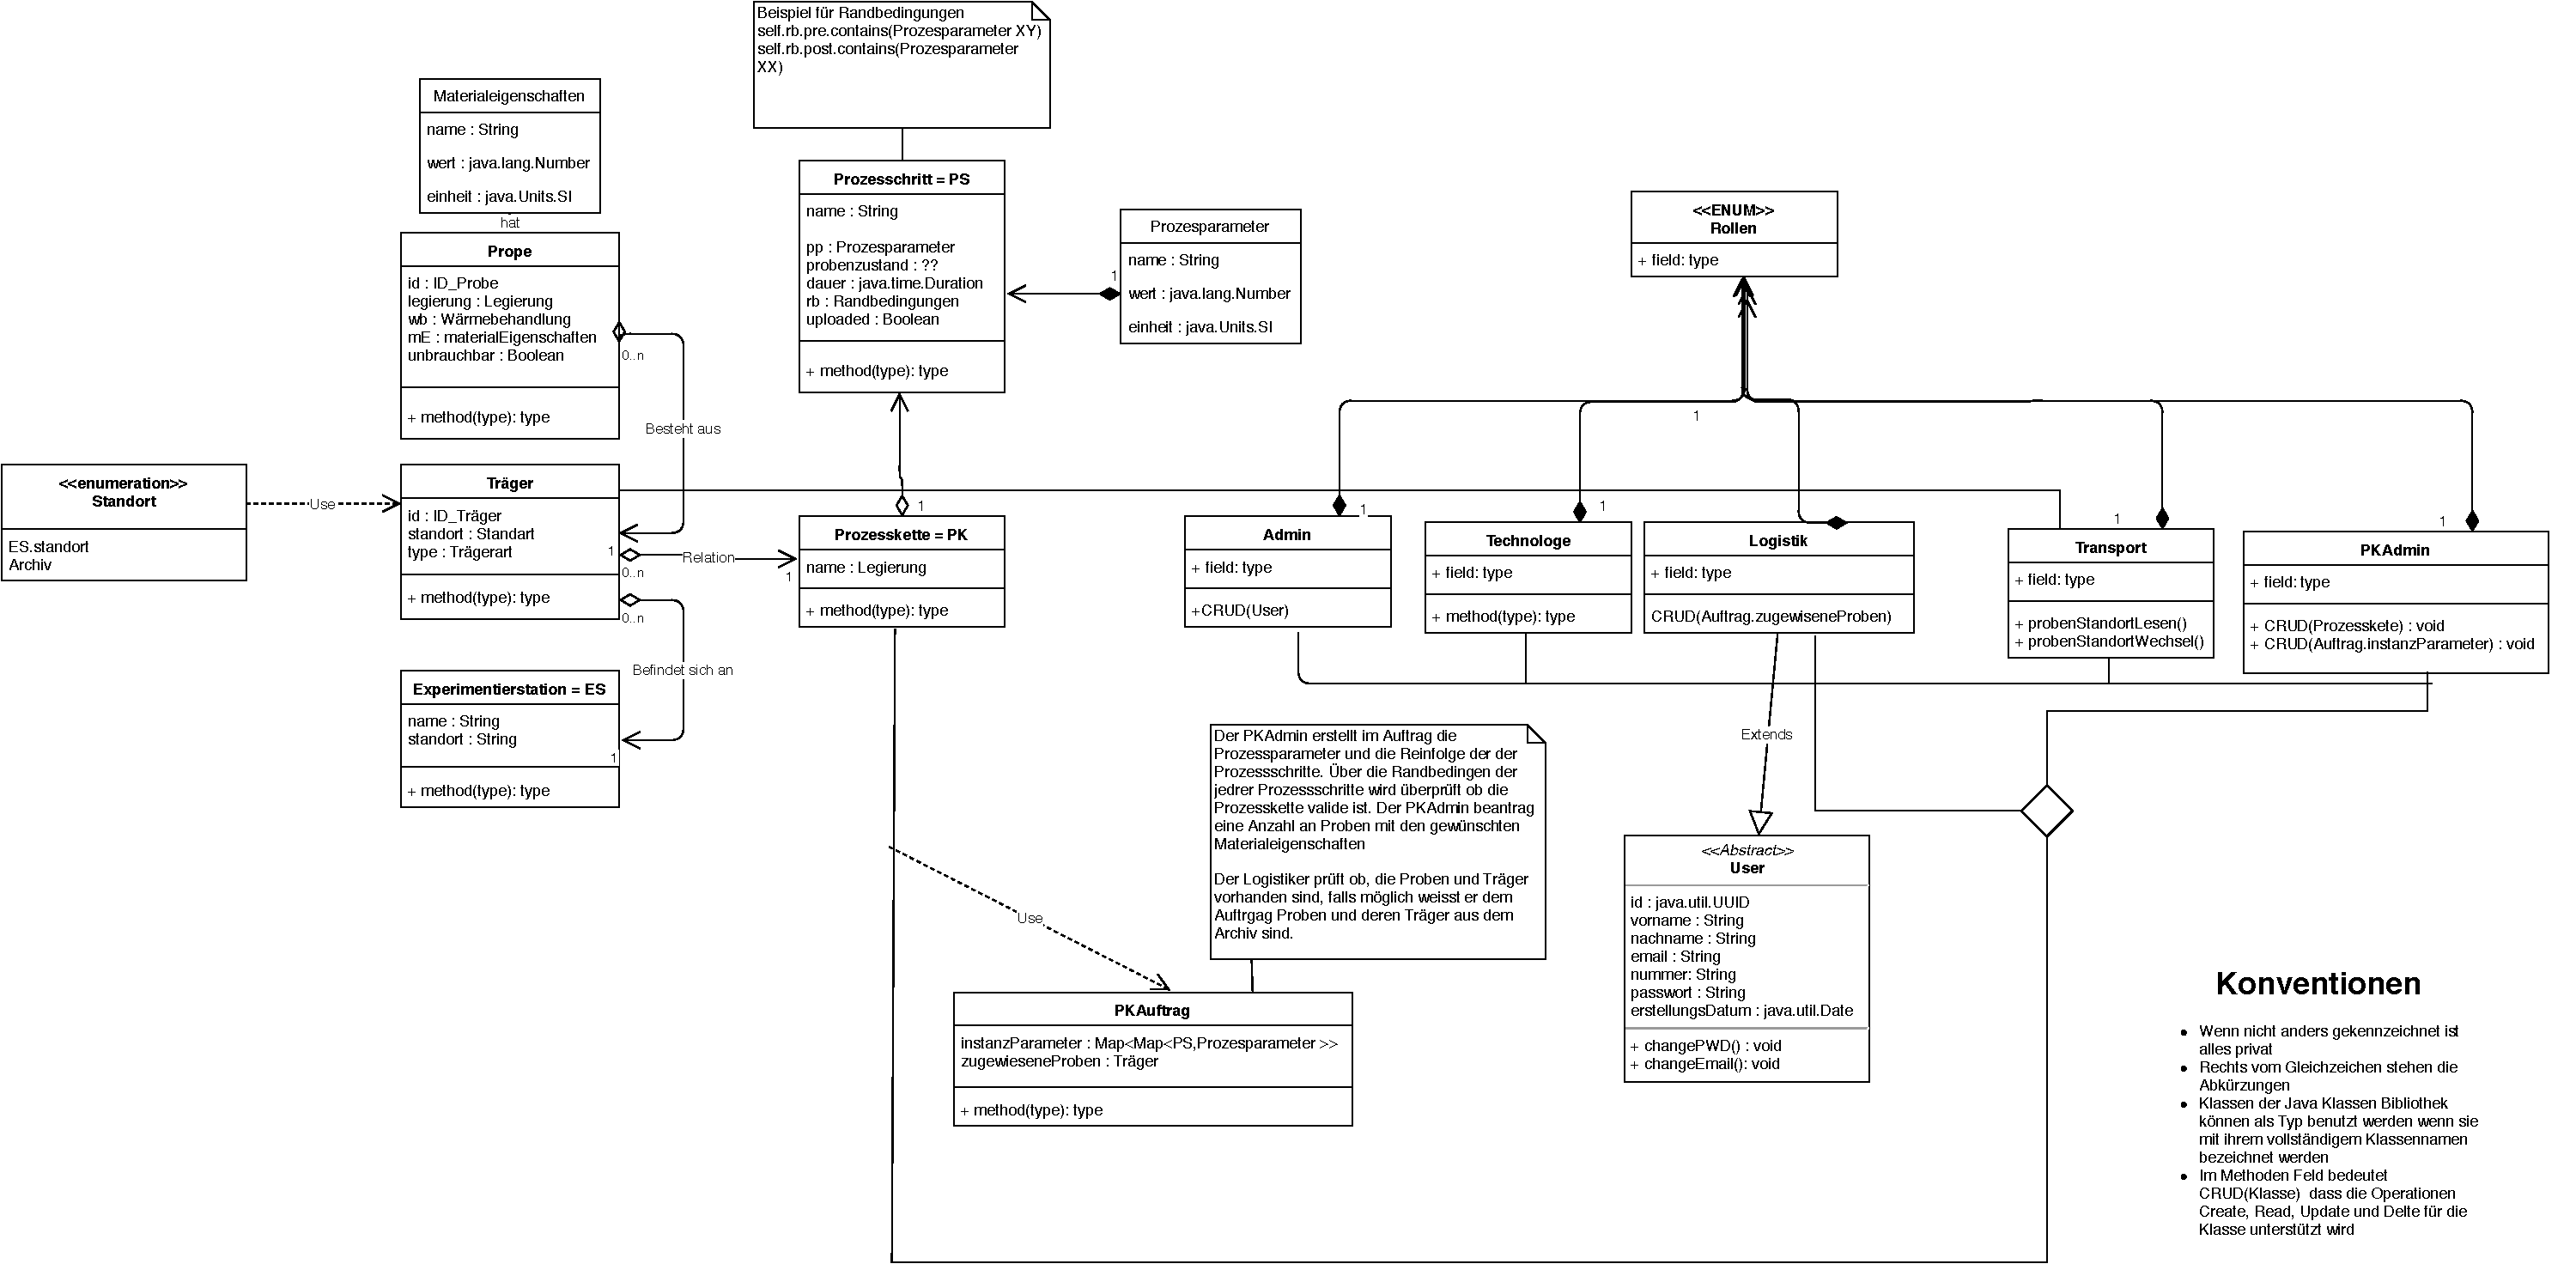
\includegraphics[width=0.75\textwidth]{UML/Model.pdf}
 \end{sidewaysfigure}

\section{Ausführungssicht}

\label{sec:ausfuehrung}

<<<<<<< HEAD
{ Im folgenden Schritt werden wir die Ausführungssicht erläutern. Es wird aufgezeigt, welche verschiedenen Geräte benötigt werden, welche Prozesse auf den Geräten jeweils laufen und welche Module dort enthalten sind.
}


%%\includepdf[]{06Ausfuehrungssicht.pdf}
\includegraphics[scale=0.5]{UML/06Ausfuehrungssicht.pdf}


{ Die Ausführungssicht von unserer Software (SWP2) ist in der obrigen Abbildung 6.1 modelliert.

Beliebig viele Benutzer können via TCP/IP auf den SFB-Server zugreifen. Dies geschieht über eine Webapplikation, die im Internetbrowser eines PCs oder eines mobilen Endgerät läuft.

Es gibt einen Anwendungsserver, welchen wir SFB-Server genannt haben, auf dem eine Instanz von Wildfly läuft. Auf dieser Wildflyinstanz wird der SWP2-Server mit allen dazugehörigen modulen ausgeführt.

Der SFB-Server stellt eine Verbindung über TCP/IP eine Verbindung zu dem einzigen Datenbankserver her. Auf dem Server läfut eine Instanz der Datenbanksoftware (........INSERT NAME...........).

}

=======
>>>>>>> docEinleitung
{\it
Die Ausführungssicht beschreibt das Laufzeitverhalten. Hier
werden die Laufzeitelemente aufgeführt und beschrieben, welche Module
sie zur Ausführung bringen. Ein Modul kann von mehreren
Laufzeitelementen zur Laufzeit verwendet werden. Die Ausführungssicht
beschreibt darüber hinaus, welche Laufzeitelemente spezifisch
miteinander kommunizieren. Zudem wird bei verteilten Systemen
(z.\,B. Client-Server-Systeme) dargestellt, welche Module von welchen
Prozessen auf welchen Rechnern ausgeführt werden.}


\section[Zusammenhänge zwischen Anwendungsfällen und Architektur]{Zusammenhänge zwischen Anwendungsfällen und Architektur\sectionmark{Zusammenhänge AF u. Architektur}}
\sectionmark{Zusammenhänge AF u. Architektur}
\label{sec:anwendungsfaelle}

{\it In diesem Abschnitt sollen Sequenzdiagramme mit Beschreibung(!)
  für zwei bis drei von Euch ausgewählte
    Anwendungsfälle
  erstellt werden. Ein Sequenzdiagramm beschreibt den
  Nachrichtenverkehr zwischen allen Modulen, die an der Realisierung
  des Anwendungsfalles beteiligt sind.  Wählt die
    Anwendungsfälle so, dass nach Möglichkeit alle Module Eures
    entworfenen Systems in mindestens einem Sequenzdiagramm
    vorkommen. Falls Euch das nicht gelingt, versucht möglichst viele
    und die wichtigsten Module abzudecken. }

\section{Evolution}

\label{sec:evolution}

{\it
  Beschreibt in diesem Abschnitt, welche Änderungen Ihr
  vornehmen müsst, wenn sich Anforderungen oder Rahmenbedingungen
  ändern. Insbesondere würden hierbei die in der
  Anforderungsspezifikation unter "`Ausblick"' genannten
  Punkte behandelt werden.}

\dots


\end{document}


%%% Local Variables:
%%% mode: latex
%%% mode: reftex
%%% mode: flyspell
%%% ispell-local-dictionary: "de_DE"
%%% TeX-master: t
%%% End:
